\documentclass[convert={size=600x1300,outext=.jpg},class=minimal,border=0mm]{standalone}
\usepackage{tikz}
\usetikzlibrary{backgrounds}
\usetikzlibrary{patterns}
\begin{document}
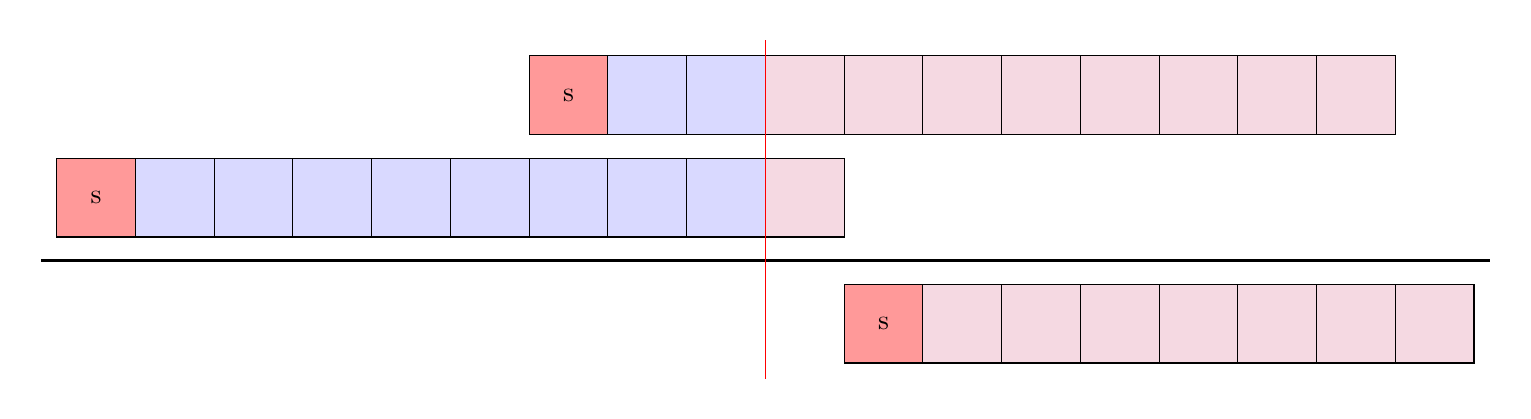
\begin{tikzpicture}[ show background rectangle, background rectangle/.style={fill=white} ]

	\tikzstyle{fractional}=[fill=red!40]
	\tikzstyle{integer}=[fill=blue!15]
	\tikzstyle{sign}=[fill=purple!15]

	%FPF=(2,-8)
	\draw (-2.000000,0.000000) rectangle ++(1,1) [fill=red!40,] node[midway] {s};
	\draw (-1.000000,0.000000) rectangle ++(1,1) [fill=blue!15,] node[midway] {};
	\draw (0.000000,0.000000) rectangle ++(1,1) [fill=blue!15,] node[midway] {};
	\draw (1.000000,0.000000) rectangle ++(1,1) [fill=purple!15,] node[midway] {};
	\draw (2.000000,0.000000) rectangle ++(1,1) [fill=purple!15,] node[midway] {};
	\draw (3.000000,0.000000) rectangle ++(1,1) [fill=purple!15,] node[midway] {};
	\draw (4.000000,0.000000) rectangle ++(1,1) [fill=purple!15,] node[midway] {};
	\draw (5.000000,0.000000) rectangle ++(1,1) [fill=purple!15,] node[midway] {};
	\draw (6.000000,0.000000) rectangle ++(1,1) [fill=purple!15,] node[midway] {};
	\draw (7.000000,0.000000) rectangle ++(1,1) [fill=purple!15,] node[midway] {};
	\draw (8.000000,0.000000) rectangle ++(1,1) [fill=purple!15,] node[midway] {};

	%FPF=(8,-1)
	\draw (-8.000000,-1.300000) rectangle ++(1,1) [fill=red!40,] node[midway] {s};
	\draw (-7.000000,-1.300000) rectangle ++(1,1) [fill=blue!15,] node[midway] {};
	\draw (-6.000000,-1.300000) rectangle ++(1,1) [fill=blue!15,] node[midway] {};
	\draw (-5.000000,-1.300000) rectangle ++(1,1) [fill=blue!15,] node[midway] {};
	\draw (-4.000000,-1.300000) rectangle ++(1,1) [fill=blue!15,] node[midway] {};
	\draw (-3.000000,-1.300000) rectangle ++(1,1) [fill=blue!15,] node[midway] {};
	\draw (-2.000000,-1.300000) rectangle ++(1,1) [fill=blue!15,] node[midway] {};
	\draw (-1.000000,-1.300000) rectangle ++(1,1) [fill=blue!15,] node[midway] {};
	\draw (0.000000,-1.300000) rectangle ++(1,1) [fill=blue!15,] node[midway] {};
	\draw (1.000000,-1.300000) rectangle ++(1,1) [fill=purple!15,] node[midway] {};

	%result
	%FPF=(-2,-9)
	\draw (2.000000,-2.900000) rectangle ++(1,1) [fill=red!40,] node[midway] {s};
	\draw (3.000000,-2.900000) rectangle ++(1,1) [fill=purple!15,] node[midway] {};
	\draw (4.000000,-2.900000) rectangle ++(1,1) [fill=purple!15,] node[midway] {};
	\draw (5.000000,-2.900000) rectangle ++(1,1) [fill=purple!15,] node[midway] {};
	\draw (6.000000,-2.900000) rectangle ++(1,1) [fill=purple!15,] node[midway] {};
	\draw (7.000000,-2.900000) rectangle ++(1,1) [fill=purple!15,] node[midway] {};
	\draw (8.000000,-2.900000) rectangle ++(1,1) [fill=purple!15,] node[midway] {};
	\draw (9.000000,-2.900000) rectangle ++(1,1) [fill=purple!15,] node[midway] {};

	\draw (-8.200000,-1.600000) -- (10.200000,-1.600000) [color=black,line width=1pt];

	\draw (1.000000,1.200000) -- (1.000000,-3.100000) [color=red];

\end{tikzpicture}
\end{document}